\usepackage{amsmath}
\usepackage{graphicx}
\usepackage{booktabs}
\usepackage{tabularx}
\usepackage{tikz}
\usetikzlibrary{arrows.meta,positioning}
\usepackage{hyperref}
\section{Solicitud clínica y alcance}

El proyecto responde a la necesidad de revisar registros EEG
prolongados y describir cambios de amplitud, actividad rítmica
y distribución espectral alrededor de crisis anotadas.
El dashboard permite navegar el trazado, revisar su calidad
y comparar segmentos ictales con segmentos sin crisis anotada.

El sistema constituye un prototipo de revisión retrospectiva.
No demuestra diagnóstico, predicción de crisis, localización
de un foco causal ni respuesta terapéutica. Un segmento sin
crisis anotada no representa un control sano.

\section{Fundamento fisiológico}

El EEG de superficie refleja principalmente la suma espacial
y temporal de corrientes postsinápticas de poblaciones
corticales con geometría favorable. La orientación neuronal,
la coordinación temporal y la conducción de volumen
influyen en los potenciales registrados. El EEG no representa
directamente la descarga de una sola neurona.

Las derivaciones del registro son bipolares: cada canal
representa una diferencia de potencial entre dos electrodos.
Por ejemplo:

\[
V_{\mathrm{FP1-F7}} = V_{\mathrm{FP1}}-V_{\mathrm{F7}}.
\]

La amplitud y polaridad dependen de ambos electrodos.
Una diferencia pequeña no demuestra ausencia de actividad.
La similitud entre canales con electrodos compartidos tampoco
demuestra conectividad neuronal. No se construyen directamente
topografías de potenciales de electrodos a partir de estas
diferencias bipolares.

Durante una crisis pueden aparecer cambios de amplitud,
patrones rítmicos y redistribución espectral. Sin embargo,
el movimiento y los parpadeos pueden aumentar componentes
lentas, mientras que la actividad muscular puede aumentar
amplitud, longitud de línea y potencia rápida. Los indicadores
deben interpretarse junto con el trazado y la calidad.

\section{Datos y adquisición}

Se utilizó CHB-MIT Scalp EEG Database, versión 1.0.0,
publicada en PhysioNet bajo Open Data Commons Attribution
License v1.0. Se descargaron el registro
\texttt{chb01\_03.edf} y el resumen oficial
\texttt{chb01-summary.txt}.

\begin{table}[htbp]
\centering
\caption{Características verificadas del registro.}
\begin{tabular}{ll}
\toprule
Característica & Resultado \\
\midrule
Frecuencia por canal & 256 Hz \\
Duración & 3600 s \\
Muestras por canal & 921\,600 \\
Canales almacenados & 23 \\
Unidad física declarada & $\mu$V \\
Crisis anotadas & 1 \\
Inicio y final & 2996--3036 s \\
Duración de la crisis & 40 s \\
Intervalo de revisión & 2876--3156 s \\
\bottomrule
\end{tabular}
\end{table}

La crisis y el intervalo de revisión están dentro de la duración
del registro. Todos los tiempos se conservan en segundos desde
el inicio del EDF. Las fechas del EDF fueron sustituidas para
proteger la privacidad y no se interpretan como fechas clínicas.

\subsection{Cadena de adquisición}

\begin{figure}[htbp]
\centering
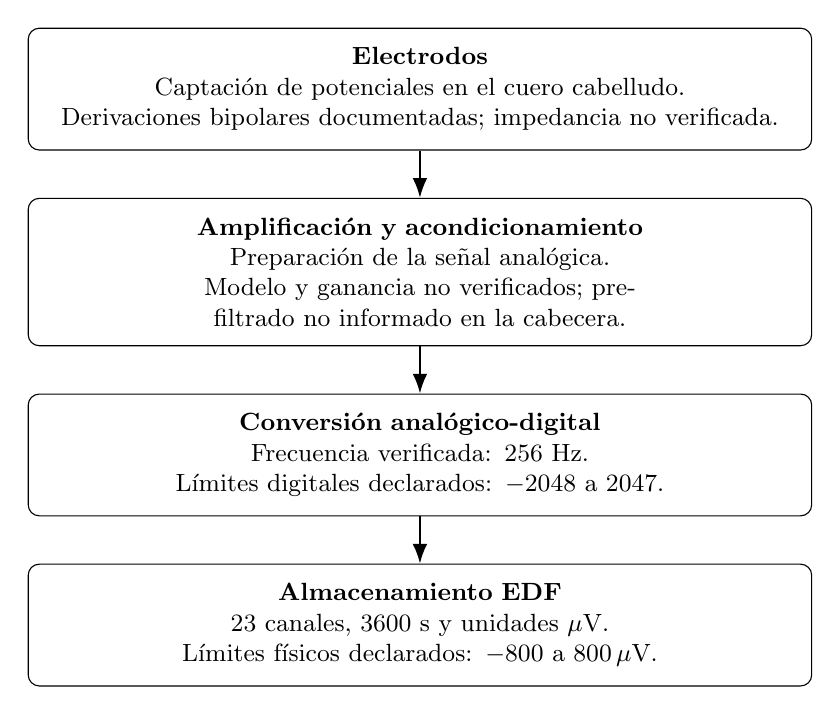
\begin{tikzpicture}[
    node distance=6mm,
    stage/.style={
        draw,
        rounded corners,
        align=center,
        text width=0.78\linewidth,
        inner sep=7pt,
        font=\small
    },
    flow/.style={-{Latex[length=2.5mm]},thick}
]
\node[stage] (electrodes) {
    \textbf{Electrodos}\\
    Captación de potenciales en el cuero cabelludo.\\
    Derivaciones bipolares documentadas;
    impedancia no verificada.
};

\node[stage,below=of electrodes] (amplifier) {
    \textbf{Amplificación y acondicionamiento}\\
    Preparación de la señal analógica.\\
    Modelo y ganancia no verificados;
    prefiltrado no informado en la cabecera.
};

\node[stage,below=of amplifier] (adc) {
    \textbf{Conversión analógico-digital}\\
    Frecuencia verificada: 256 Hz.\\
    Límites digitales declarados: $-2048$ a $2047$.
};

\node[stage,below=of adc] (edf) {
    \textbf{Almacenamiento EDF}\\
    23 canales, 3600 s y unidades $\mu$V.\\
    Límites físicos declarados: $-800$ a $800\,\mu$V.
};

\draw[flow] (electrodes) -- (amplifier);
\draw[flow] (amplifier) -- (adc);
\draw[flow] (adc) -- (edf);
\end{tikzpicture}
\caption{Cadena conceptual de adquisición. Los parámetros
indicados proceden de la auditoría del EDF; el esquema
no representa un circuito verificado del hardware original.}
\label{fig:acquisition}
\end{figure}

Los 23 canales declaran límites físicos de
$-800$ a $800\,\mu$V y digitales de $-2048$ a $2047$.
La escala física declarada es:

\[
q=\frac{800-(-800)}{2047-(-2048)}
=\frac{1600}{4095}
\approx 0.390720391\,\mu\mathrm{V/código}.
\]

La documentación del dataset indica una resolución de
16 bits. El rango digital declarado contiene 4096 códigos,
pero no permite determinar por sí solo la resolución
del ADC original.

El campo de prefiltrado está vacío: no informa los filtros
de adquisición y no demuestra su ausencia. Los límites
de cabecera tampoco demuestran saturación; deben contrastarse
con las muestras.

MNE entrega las señales EEG en voltios. El código convierte
una sola vez a microvoltios mediante el factor $10^6$.

\subsection{Trazabilidad}

El manifiesto conserva nombre, versión, URL, fecha de
descarga, ruta relativa, tamaño y SHA-256 de ambos archivos.

El EDF se descargó el 7 de octubre de 2026 a las
02:20:28 UTC, con tamaño de 42\,399\,744 bytes.
El resumen se descargó a las 02:20:29 UTC,
con tamaño de 5355 bytes. Ambas descargas corresponden
al 6 de octubre en Colombia.

Las huellas permiten detectar cambios respecto al contenido
registrado; no se contrastaron con una huella oficial
independiente.

\subsection{Montaje y redundancias}

Los 23 nombres originales coinciden, en nombre y orden,
con el montaje del resumen oficial. No se identificaron
canales ficticios denominados ``-'' ni canales no EEG
en la lista de este registro.

Se compararon las 921\,600 muestras de los pares
potencialmente redundantes:

\begin{itemize}
    \item \texttt{T8-P8-0} y \texttt{T8-P8-1} fueron idénticos,
    con diferencia máxima y RMSE de $0\,\mu$V.
    Se conserva \texttt{T8-P8-0}.
    \item \texttt{T7-P7} y \texttt{P7-T7} presentaron
    polaridad invertida y desplazamiento constante:
\end{itemize}

\[
x_{\mathrm{P7-T7}}
=-x_{\mathrm{T7-P7}}+0.390720391\,\mu\mathrm{V}.
\]

La desviación estándar de su suma fue aproximadamente
$4.67\times10^{-15}\,\mu$V. Se conserva
\texttt{T7-P7} y se excluye \texttt{P7-T7} por redundancia.

Quedan 21 derivaciones candidatas tras las exclusiones.
Esta decisión no demuestra buena calidad en todos los canales.
El EDF original se conserva completo.

\section{Justificación de los indicadores}

\begin{table}[htbp]
\centering
\small
\caption{Relación entre indicadores, necesidad y límites.}
\begin{tabularx}{\linewidth}{@{}p{0.23\linewidth}XX@{}}
\toprule
Indicador & Utilidad & Límite interpretativo \\
\midrule
RMS centrado ($\mu$V)
& Describe amplitud respecto a la media.
& Depende del montaje y puede aumentar por artefactos. \\

Longitud de línea media ($\mu$V)
& Describe variación entre muestras consecutivas.
& Depende del muestreo y filtro; sensible a actividad muscular. \\

Potencia absoluta ($\mu$V$^2$)
& Describe potencia integrada por banda.
& Las bandas aisladas no demuestran crisis. \\

Potencia relativa (fracción o \%)
& Describe proporción de potencia por banda.
& Depende del denominador; puede aumentar aunque la absoluta disminuya. \\

Entropía espectral (sin unidad)
& Describe concentración o dispersión espectral.
& Depende de resolución y ruido; puede subir o bajar durante una crisis. \\

Duración y fracción ictal (s y \%)
& Cuantifican tiempo cubierto por anotaciones.
& No representan detección automática. \\

Banderas de calidad
& Identifican segmentos que requieren revisión.
& No confirman automáticamente artefactos. \\
\bottomrule
\end{tabularx}
\end{table}

Se utilizan las bandas delta de 0.5--4 Hz, theta de 4--8 Hz,
alfa de 8--13 Hz y beta de 13--30 Hz. El denominador de
potencia relativa comprende 0.5--40 Hz, incluida la potencia
de 30--40 Hz, que no representa toda la banda gamma.

Una señal de potencia total nula produce potencia relativa
y entropía indefinidas; deben registrarse como valores ausentes.
Las ecuaciones y parámetros de cálculo se documentan en
la sección de métodos del equipo.

\section{Inspección visual inicial}

Se revisaron las derivaciones \texttt{FP1-F7},
\texttt{F7-T7}, \texttt{FP2-F8} y \texttt{F8-T8},
con escala común de amplitud y anotaciones oficiales.
No se aplicó filtrado por el equipo en estas figuras.

Se observaron cambios de amplitud y morfología alrededor
de la crisis, con diferencias entre derivaciones.
Persistieron oscilaciones y transitorios después del final
anotado de 3036 s.

El intervalo 3070--3080 s presentó una deflexión lenta
hacia 3073 s y oscilaciones rápidas hacia 3075--3076 s.
Se propone revisarlo con el módulo de calidad, sin clasificarlo
automáticamente como artefacto ni como otra crisis.

En las capturas no se aprecia señal plana prolongada
ni recorte evidente. Esto no descarta anomalías breves
ni demuestra buena calidad de todo el registro.
La revisión se limita a cuatro canales y a los segmentos
seleccionados.

\section{Conclusión de la auditoría}

Se verificaron estructura, montaje, unidades, frecuencia
y anotaciones del registro, conservando su origen temporal.
Se documentaron dos redundancias y sus exclusiones propuestas.
La cabecera aportó límites de conversión y dejó el prefiltrado
sin informar. La interpretación posterior debe combinar
indicadores, trazado y evaluación completa de calidad.

\subsection*{Fuentes de esta sección}

\begin{itemize}
    \item Guttag, J. (2010).
    \textit{CHB-MIT Scalp EEG Database}, versión 1.0.0.
    PhysioNet.
    \url{https://doi.org/10.13026/C2K01R}.
    \item Caicedo-Rodríguez, P. E.
    \textit{EEG y revisión de crisis epilépticas}.
    Guía docente del laboratorio.
    \url{https://pablocaicedor.github.io/laboratorios/SBVI/laboratorio_EEG_completo/laboratorio_EEG.html}.
    \item Resumen oficial \texttt{chb01-summary.txt}
    y resultados de auditoría del proyecto.
    \item MNE-Python. Documentación de lectura EDF.
    \url{https://mne.tools/stable/generated/mne.io.read_raw_edf.html}.
\end{itemize}